\chapter{Introduction}
\label{ch:introduction}
Increased competition and complexity of the problems companies are solving today is changing how software is developed. Software development is getting increasingly more focused towards having short and independent release cycles based on individual features rather than entire applications. Solving complex problems often yield a very complex and fragile solution, but the most successful tech companies have succeeded in utilizing a new architecture pattern: Microservices. By creating microservices, changing development process and team structure drastically, modern tech companies create innovative and resilient software quicker than ever seen before.

Several factors has made this new paradigm for developing big scale distributed applications possible. Cloud computing has made it possible to buy computing resources as they are needed, cheap and fast. Virtualization and lately containerization making it possible to create isolated environments, enabling partitioning of applications, into a subset of components that can be developed and deployed independently. The possibility to dynamically orchestrate containers, and ensuring correct capacity and redundancy of application components automatically. Segmentation of the applications in turn makes it possible to maintain a acceptable level of complexity of the source code improving maintainability and increasing agility.

\note {
A boom of knowledge sharing throughout the industry, through conference talks and a huge variety of high quality open source projects, together with new programming languages, makes it possible for independent development teams to go from development to deployment very quickly, while taking the complexity of the internet increasingly into account. This has created a new and competitive environment, where understanding and solving complex problems is a process that has to be repeated daily and quickly. Software developers now need to understand the domain and the context they are developing software for in a much higher degree than ever before. 
Having the best and most stable solution to a given problem is not necessarily enough, time to market is extremely important to capture market share as well. New applications need to be available to the customer immediately, and at all times, lack of new features and downtime is immediately visible on the company bottom line.
}

\section{Microservices}
Monolith applications were a result of technological boundaries, and made developing good design a major challenge. These boundaries have disappeared, pushing developers towards more thoughtful design of applications. Developers today need to put emphasis on understanding the underlying challenges in the particular domain, identifying the optimal architecture that supports the context\cite{evans2016tackling}. High complexity and a strict time to market makes problem solving hard. It is therefore very important to optimize the entire process from identification of a correct solution, through development and deployment of the feature. There are three clear factors in this process: technology utilization, correct working process and organisational structure\cite{george2016it}. Traditionally speaking organisations often divided people into departments according to their specific competences. Each department would be a separated unit, where everyone had the same competences. A new development project would therefore span several departments, creating a need for standardization of tools, languages and working processes. This inherently limits the amount of innovation possible, engineers are forced to solve a problem with a predetermined process, often resulting in similar solutions for very diverse problems\cite{george2016it}. 
Many tech companies have publicly talked about their innovative ways of working, that has allowed them to improve the amount of innovation and the throughput of their software engineers\cite{kniberg2014spotify}. By having a strong focus on having small, strong, cross-functional and self-organising teams that have "end-to-end" responsibility for the features they build. Teams have a overall mission, knowledge of their specific product strategy and short-term goals that help keep the team on the wished path. Each team is given autonomy, responsible for finding the best way for the team to develop new features, which features the team should implement and how they work together. Everyone in the team is located in the same physical location, creating the optimal conditions for good collaboration across skill-sets\cite{kniberg2014spotify}.


\begin{figure}[!htb]
  \begin{center} 
	  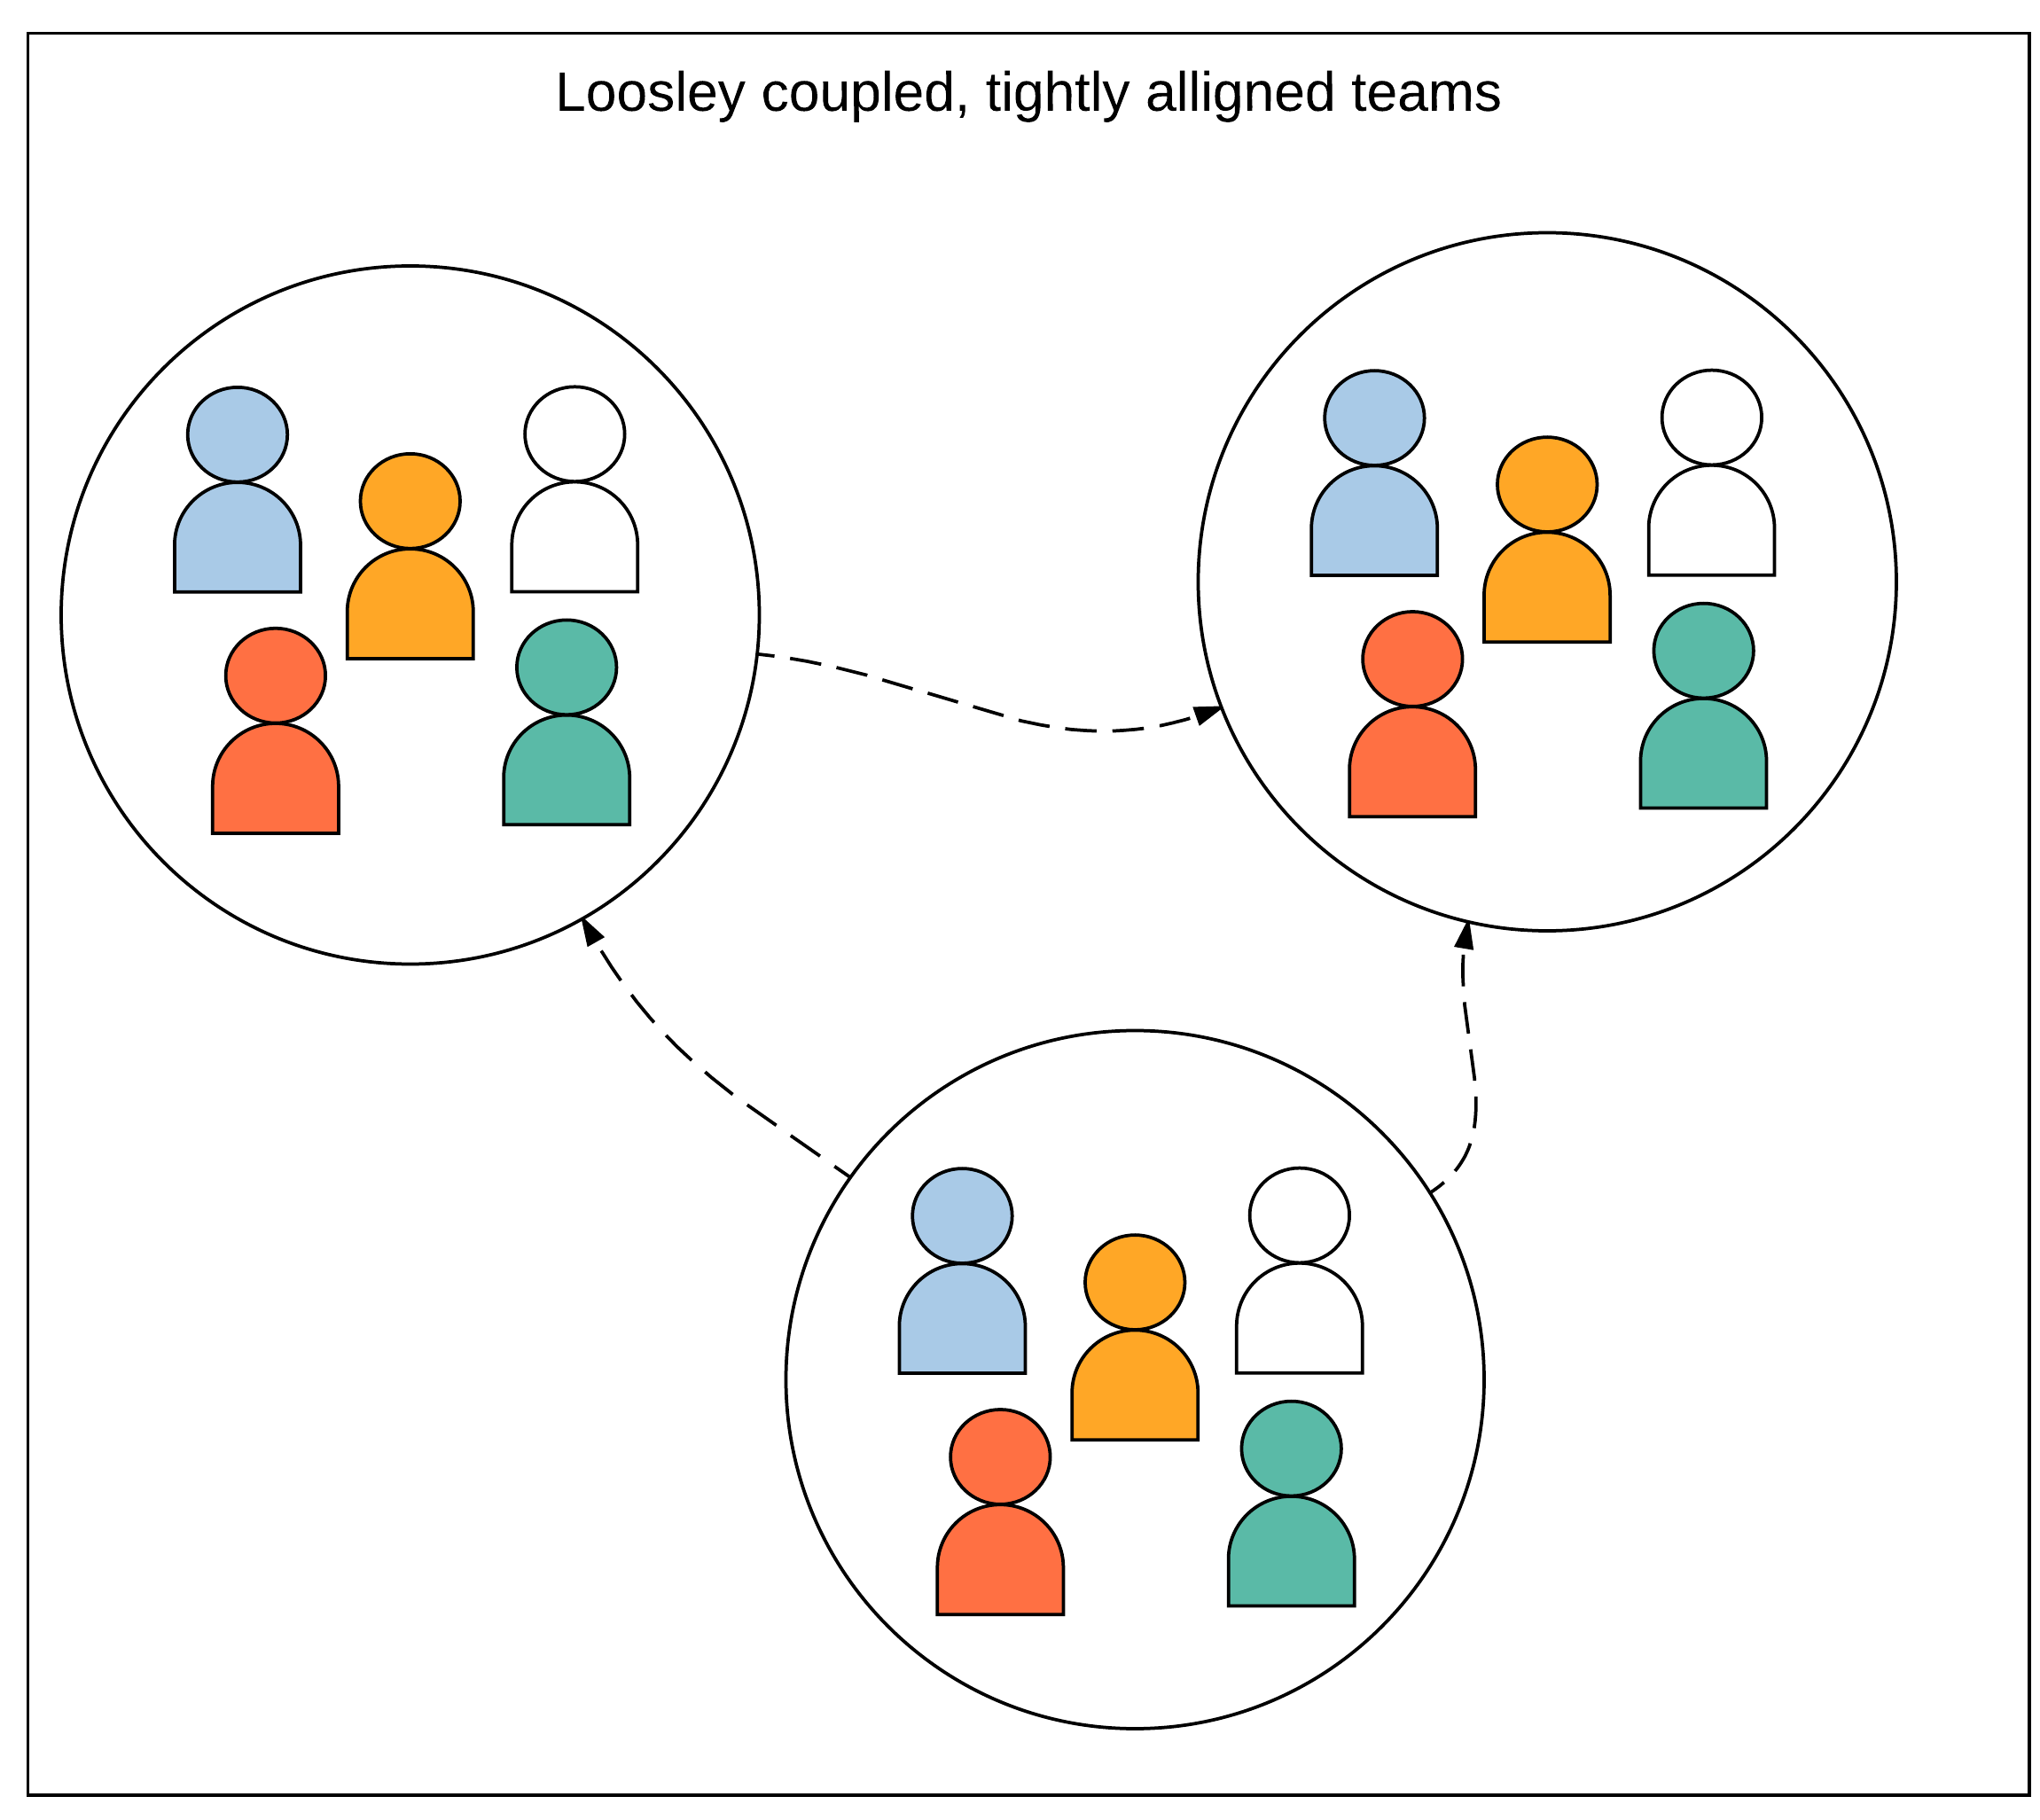
\includegraphics[scale=0.27]{introduction_squads}  
  \end{center}
  \caption{Spotify team structure}
  \label{fig:introduction_squads}
\end{figure}

This is a completely new way of designing a organisation, and removes pre-existing process and organisation inhibitors. It is possible for each team to create and release features independently, minimizing waiting time between teams. At the same time teams are responsible for what they create, removing handoffs between teams. The focus is having loosely coupled but tightly aligned teams\cite{kniberg2014spotify}.
It is important that organisation and process inhibitors are removed before utilizing microservices as an architecture choice\cite{meshenberg2016microservices}. This will make it possible to utilize available technology to the fullest, by allowing teams to choose which technology is used for development of the separate features\cite{fowler2014polyglot}. A central database slows down teams, by creating dependencies across team boundaries, creating a need for coordinating changes. Giving the possibility for a polyglot database architecture where a specific database technology is used because of it's advantages in the specific situation creating a system that contains several databases with different data\cite{george2016it, fowler2014microservices}.

\comment{Increase focus on the technology aspect, it is after all our main interest}

\section{Knowledge sharing}
A huge trend of knowledge sharing has started, where online accessible conference talks and a high quantity of open source projects inspire and help developers solve common challenges. Conferences have focus on new open source technology, system architecture, working process and organisational structure, all with a common goal: speeding up software development and the ability to solve increasingly difficult problems. Conferences are either entirely committed to or has tracks about topics like: Cloud computing, Agile development, Domain Driven Design, Microservices, NoSQL, Docker, Cassandra among many others\cite{george2016it}. Company internal projects that beforehand was only internal accessible, are increasingly made open source, giving developers very advanced tools to create elegant and efficient solutions quickly. These projects are freely accessible, with well known support challenges, where developers can find help with specific challenges utilizing the projects.

The entire movement started when Amazon announced Amazon Web Services in 2006. It meant anyone could register and rent virtual machines for hosting distributed applications. Since then, virtualization has been further revolutionised with the introduction of container technology, which was made open source through the docker initiative in 2014. Docker made it possible to start up new independent and isolated environments in seconds, something Google had developed on internally because they needed it\cite{bernstein2014containers}. Which is somewhat a trademark for the entirety of the cloud native movement, is has sprung out of a big variety of needs: serving massive amounts of users, creating reliable applications, the ability to update and add functionality often and easily, minimize integration complexity and technology lock in. In the end the focus should be on solving the problems at hand and in the future, not maintenance and effects of new extensions on the existing application.



"In a post-GitHub world, it is no longer sufficient for a software foundation to offer just a software repo, mailing list, and website: we need to offer an enhanced set of services that facilitates increased adoption. You should host your project with the Cloud Native Computing Foundation (CNCF) becaus"

\url{https://www.cncf.io/projects/}

\section{Resilience}
%Fail whale \url{http://www.whatisfailwhale.info/}
\note {
Distanced view on deployment, focus on development phase
High requirements for availability, always online, always used by users
}

From preface of Newman book:

\note{
if the fundamental design of the system doesn’t make it easy to make changes, then there are limits to what can be accomplished.

At the same time, many organizations were experimenting with finer-grained architectures to accomplish similar goals, but also to achieve things like improved scaling, increasing autonomy of teams, or to more easily embrace new technologies. 
}

From chapter 1 page 1 Newman book: 
\note{

Amazon and Google espoused the view of small teams owning the full lifecycle of their services. And, more recently, Netflix has shared with us ways of building antifragile systems at a scale that would have been hard to comprehend just 10 years ago.
Domain-driven design. Continuous delivery. On-demand virtualization. Infrastruc‐ ture automation. Small autonomous teams. Systems at scale. Microservices have emerged from this world. They weren’t invented or described before the fact; they emerged as a trend, or a pattern, from real-world use.
}


The inherent problem with distributed systems is their resilience. How well do they match up against the face of disruptive events or internal errors. A lot of different errors can occur, when a application is deployed, and it is by nature very hard to reason about which error occurred and why, when the system is in production. It is near impossible to exhaust every possible error pattern through preliminary testing, especially if the application has any modest level of complexity. At the same time, the test environment will never completely match the production environment. Precautionary measures therefore need to be taken, taking into account that latent bugs, error patterns and external events will challenge any deployed application. 

With today's technology and tools available it is possible to create resilient application.

With the correct amount of benchmark testing and fail saves, it is possible to guaranty up time.

%\url{http://tech.opentable.co.uk/blog/2014/02/28/api-benchmark/}
"As developers we rely on technologies that, with a minimum effort, can guarantee some pretty decent results in terms of performance. Modern web frameworks handle concurrency and thread management without requiring much plumbing code. Sophisticated and relatively cheap cloud services help us monitor our applications, providing dashboards, reports and alerting systems. Deploying on the cloud we can run our services and even auto-scale them depending on how much power we need. Even with these tools we must still own the responsibility of writing good quality code, testing it properly, and deploying as fast as possible in order to optimise the delivery process of our products."

But what about performance? I mean, what about the relationship between the code we write every day, and the way we impact overall performance? Are we sure that we are not deploying to production something that is degrading our services’ performance?"

\comment{Expand and include references}

\note {
You do not want a single point of failure. We want to isolate failures, so we do not get cascading failures. Then redundancy does not necessarily help.
}

\note {
These requirements has started big scale initiatives in cloud computing, has generated new tools and databases available for development of distributed big scale enterprise applications. 

Creating a need for developers to explore and evaluate which of the many platforms to choose, 

has generated new tools and databases available for development of distributed big scale enterprise applications.

platform for automating deployment, scaling, and operations of application containers across clusters of hosts

Which level are we on? High level: Google app engine, or low level abstraction: EC2.

"The Antifragile Organization" - \url{http://queue.acm.org/detail.cfm?id=2499552}
"Failure is inevitable. Disks fail. Software bugs lie dormant waiting for just the right conditions to bite. People make mistakes. Data centers are built on farms of unreliable commodity hardware. If you're running in a cloud environment, then many of these factors are outside of your control. To compound the problem, failure is not predictable and doesn't occur with uniform probability and frequency. The lack of a uniform frequency increases uncertainty and risk in the system. In the face of such inevitable and unpredictable failure, how can you build a reliable service that provides the high level of availability your users can depend on?"

Why is it worth it to take on this monster of instability?


"Weathering the Unexpected" - \url{http://queue.acm.org/detail.cfm?id=2371516}

"Whether it is a hurricane blowing down power lines, a volcanic-ash cloud grounding all flights for a continent, or a humble rodent gnawing through underground fibers—the unexpected happens. We cannot do much to prevent it, but there is a lot we can do to be prepared for it. To this end, Google runs an annual, company-wide, multi-day Disaster Recovery Testing event—DiRT—the objective of which is to ensure that Google's services and internal business operations continue to run following a disaster."


Disasters happen for all kinds of systems. So lets prepare for it already in implementation.


"Site Reliability Engineering" - (page 17 in downloaded pdf)

"Software engineering has this in common with having children: the labor before the birth is painful and difficult, but the labor a er the birth is where you actually spend most of your effort. Yet software engineering as a discipline spends much more time talking about the first period as opposed to the second, despite estimates that 40–90% of the total costs of a system are incurred after birth.1"


Software systems incur a lot of work even after deployment, so lets spend some time here.

"Toward Antifragile Cloud Computing Infrastructures"\cite{abid2014toward}
"Cloud computing systems are rapidly growing in scale and complexity. They are also changing dynamically as a result of dynamic addition and removal of system components, different execution environments, common updates and upgrades, runtime repairs, mobility of devices and more. Such large-scale, complex and dynamic cloud environments are prone to failures and performance anomalies"

"Resilience and Survivability in Communication Networks: Strategies, Principles, and Survey of Disciplines"\cite{sterbenz2010resilience}
"The Internet has become essential to all aspects of modern life, and thus the consequences of network disruption have become increasingly severe. It is widely recognised that the Internet is not suciently resilient, survivable, and dependable, and that significant research, development, and engineering is necessary to improve the situation."

"Networks in general, and the Global Internet in particular, have become essential for the routine operation of businesses and to the global economy. Consumers use the Internet to access information, obtain products and services, manage finances, and communicate with one another. Businesses use the Internet to transact commerce with consumers and other businesses."


"Toward Antifragile Cloud Computing Infrastructures" "Amal Abida,b, Mouna Torjmen Khemakhema, Soumaya Marzouka, Maher Ben Jemaaa, Thierry Monteilb,c, Khalil Drirab,c"
"Cloud computing is earning an increasing popularity over traditional information processing systems for storing and processing huge volumes of data. This concept consists in offering services and resources on-demand over the Internet in the pay-as-you-go model. The Cloud infrastructure is built on modern data centers covering thousands of interconnected servers with capability of hosting a large number of applications. These data centers are often virtualized and computing resources are provisioned to the user in the form of configurable Virtual Machines (VMs)."

Stability summary chapter 6 \cite[p. 117]{nygard2007release}
"Astronomically unlikely coincidences happen daily"
"Failures are inevitable. Our systems, and those we depend on will fail in ways large and small. Stability antipatterns amplify transient events. They accelerate cracks in the system. Avoiding the antipatterns does not prevent bad things from happening, but they wull help minimize the damage when bad things do occur."


"A View of Cloud Computing"
"While the cost of over provisioning is easily measured, the cost of under provisioning is more difficult to measure yet potentially equally serious: not only do rejected users generate zero revenue, they may never come back"
"In fact, this example underestimates the benefits of elasticity, because in addition to simple diurnal patterns, most services also experience seasonal or other periodic demand variation (for example, e-commerce in December and photo sharing sites after holidays) as well as some unexpected demand bursts due to external events "
}

\note{
“1.4. Attack of the Clusters
At the beginning of the new millennium the technology world was hit by the busting of the 1990s dot-com bubble. While this saw many people questioning the economic future of the Internet, the 2000s did see several large web properties dramatically increase in scale.”
Excerpt From: “NoSQL Distilled: A Brief Guide to the Emerging World of Polyglot Persistence.” 


“One is to handle data access with sizes and performance that demand a cluster; the other is to improve the productivity of application development by using a more convenient data interaction style”
Excerpt From: pramod j. sadalage. “NoSQL Distilled: A Brief Guide to the Emerging World of Polyglot Persistence.” iBooks.
}




\newpage
\section{Problem formulation}
\label{sc:problem_formulation}

\begin{itemize}  
\item 1.a How can cloud computing be used to solve availability, performance and maintainability requirements for enterprise applications?
\item 1.b How can cloud computing be used in an enterprise application architecture?

\item 2.a How are enterprise application challenges and possible solutions affected by the application domain?
\item 2.b How does the enterprise application domain affect challenges and possible solutions?
\item 2.c How does the domain shape the challenges in a specific application architecture?
\item 2.d How does the domain and organization shape the challenges in a specific application architecture?

\item 3.a How does a distributed application architecture deal with a single point of failure?
\item 3.b How is single point of failure avoided in a distributed application architecture?

\item 3.c How is the optimal application architecture and distribution method determined and evaluated?
\item 3.d How is the enterprise application architecture determined?
\item 3.e How is the enterprise application architecture evaluated?
\end{itemize}

\subsection*{Notes}
How are the challenges and their optimal solution affected by the specific application?

What determines the optimal application architecture, database and distribution?

How is the optimal application architecture, database and distribution determined?

System architecture:
How is application data optimally stored?
How is application data optimally distributed?

How are application updates optimally executed?
How are updates 

How is the system distributed

This area has been named cloud computing, 

Big cloud computing platforms are now available, offering server rental with 

From these requirements big cloud platforms have been started, 

These requirements has started big scale initiatives in cloud computing, has generated new tools and databases available for development of distributed big scale enterprise applications. 

Creating a need for developers to explore and evaluate which of the many platforms to choose, 